\documentclass[11pt]{beamer}
\usepackage{verbatim}
\usepackage{amsmath}
\usepackage{amsthm}
\usepackage{graphics}
\usepackage{multicol}
\usepackage{color}
\usepackage{stmaryrd}
\usefonttheme[onlymath]{serif}

\title{Progess Report 10}
\date{\today}
\author{Xie Li}
\begin{document}
\maketitle

\begin{frame}\frametitle{Overview of the Progress}
\begin{itemize}
\item Termination track of SV-COMP.
\item Problem of adapting termination checking.
\item Clang/LLVM?
\end{itemize}

\end{frame}

\begin{frame}\frametitle{Termination Track}

\textbf{Input: }
\begin{itemize}

\item Yaml file: can be parsed into paths of property file and src file.

\item 
Property: \texttt{CHECK(init(main()), LTL(F end))}

\item Src: C file.
\end{itemize}

\textbf{Output: }
\begin{itemize}
\item YES + WITNESS.
\item FALSE + Counterexample.
\item UNKNOWN.
\end{itemize}



Counterexample: should be a infinite execution.



\end{frame}


\begin{frame}\frametitle{ \textsc{SVMRanker} and What is Needed?}

\begin{itemize}
\item 
\textsc{SVMRanker}  assume the input file is a single loop program.

\textsc{SV-COMP}: may contain several loops or nested calls of functions. 
\item 
\textsc{SVMRanker} originally use boogie toolchain and can only support part of program.

\textsc{Clang\&LLVM}: a more powerful toolchain with 
\end{itemize} 
\end{frame}

\begin{frame}\frametitle{Data Structures}

Python in SVMRanker: 
\begin{center}
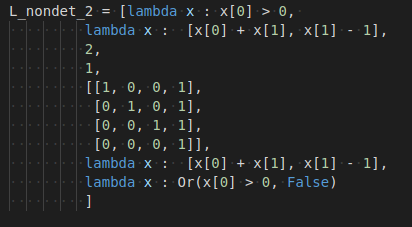
\includegraphics[scale=0.4]{pyds.png}
\end{center}

\end{frame}


\begin{frame}\frametitle{Data Structures}


IR: 
\begin{center}
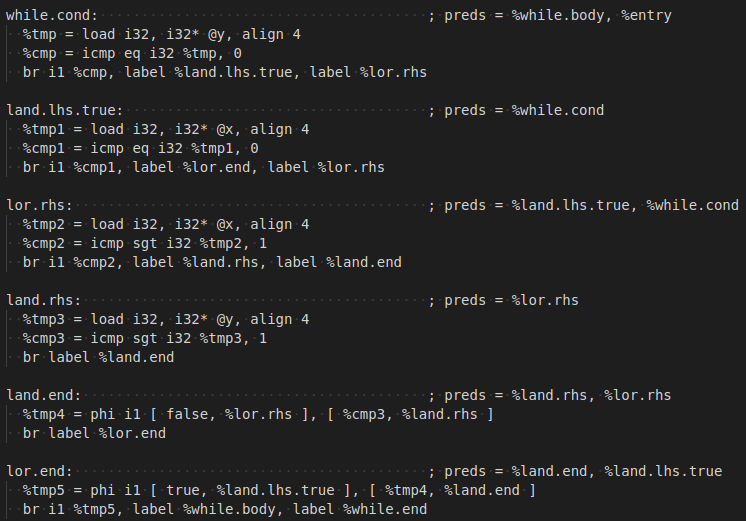
\includegraphics[scale=0.4]{ir.png}
\end{center}

\end{frame}

\begin{frame}\frametitle{Boogie Toolchain}

\end{frame}

\begin{frame}\frametitle{Currently Implemented}

\end{frame}
\end{document}